\documentclass[a4paper,12pt]{article} % добавить leqno в [] для нумерации слева
\usepackage[a4paper,top=1.3cm,bottom=2cm,left=1.5cm,right=1.5cm,marginparwidth=0.75cm]{geometry}
%%% Работа с русским языком
\usepackage{cmap}					% поиск в PDF
\usepackage{mathtext} 				% русские буквы в фомулах
\usepackage[T2A]{fontenc}			% кодировка
\usepackage[utf8]{inputenc}			% кодировка исходного текста
\usepackage[english,russian]{babel}	% локализация и переносы

\usepackage{graphicx}
\usepackage{mathtools}
\usepackage{wrapfig}
\usepackage{tabularx}
\usepackage{amssymb}
\usepackage{hyperref}
\usepackage[rgb]{xcolor}
\hypersetup{colorlinks=true,urlcolor=blue}
%% Шрифты
\usepackage{euscript}	 % Шрифт Евклид
\usepackage{amsmath}
\usepackage{mathtools}
%%% Заголовок
\author{Lokhmatov Arseniy}
\title{Лабораторная работа по общей физике}

\date{\today}
\begin{document}
\begin{titlepage}
    \newpage
    \begin{center}
    {\large МОСКОВСКИЙ ФИЗИКО-ТЕХНИЧЕСКИЙ ИНСТИТУТ (НАЦИОНАЛЬНЫЙ ИССЛЕДОВАТЕЛЬСКИЙ УНИВЕРСИТЕТ)}
    \vspace{1cm}

    {\largeФизтех-школа аэрокосмических технологий}
    \vspace{6em}
    \end{center}
    
    \vspace{1.2em}

    \begin{center}
    %\textsc{\textbf{}}
    \Large Лабораторная работа №3.7.1 \\
    Скин эффект в полом цилиндре
    \linebreak
    \end{center}
    
    \vspace{11em}
    
    \begin{flushright}
                       {\large Работу выполнили\\
                       Лохматов Арсений Игоревич\\
                       Козярский Алексей Сергеевич\\
                       Б03-303 }
    \end{flushright}

    \vspace{\fill}

    \begin{center}
        
\includegraphics[width=0.2\linewidth]{dasr.png}
    \end{center}

    \begin{center}
    Долгопрудный, 2024
    \end{center}

    \end{titlepage}

\section{Теоретическая часть}

\paragraph{Цель работы:} исследования проникновения переменного магнитного поля в медный полый цилиндр.

\paragraph{Оборудование:} генератор звуковой частоты, соленоид, намотанный на полый цилиндрический каркас из диэлектрика, медный экран в виде трубки, измерительная катушка, амперметр, вольтметр, осциллограф.

\subsection{Теоретическая часть}

В работе изучается скин-эффект в длинном тонкостенном медном цилиндре, помещённом внутрь соленоида. Теоретически такая задача сложнее, чем скин-эффект в полубесконечном пространстве: здесь требуется совместное решение уравнений скин-эффекта (уравнения диффузии поля) в стенке цилиндра и квазистационарных уравнений поля в его полости.

\begin{wrapfigure}[18]{r}{0.3\textwidth}
    \begin{center}
    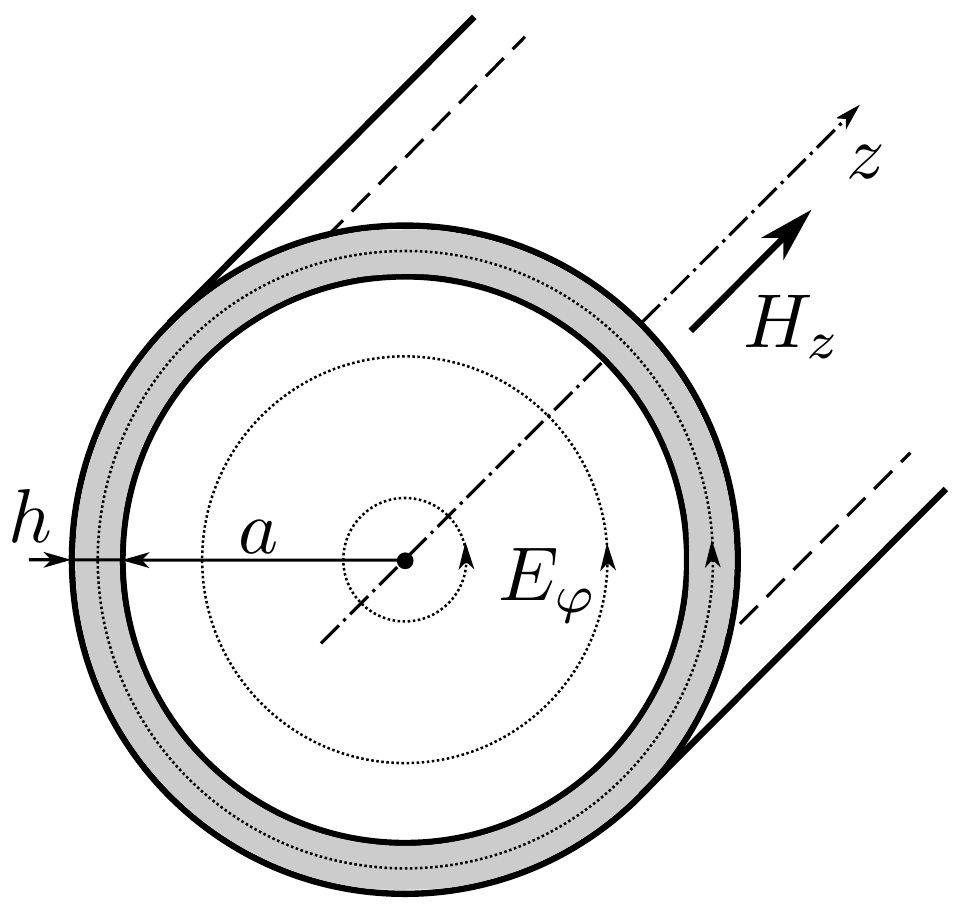
\includegraphics[width=0.28\textwidth]{cilindr}
\end{center}
\label{img1}
\caption{Электрическое и магнитное в тонкостенном цилиндре}
\end{wrapfigure}

Пусть цилиндр достаточно длинный, так что в нём можно пренебречь краевыми эффектами. В этом приближении магнитное поле $\textbf{H}$ всюду направлено по оси системы (ось $\textit{z}$), а вихревое электрическое поле $\textbf{E}$ будет всюду перпендикулярно радиусу, то есть линии поля образуют соосные окружности (рис. \ref{img1}). Все величины будем считать колеблющимися по гармоническому закону с некоторой частотой $\omega$, задаваемой частотой колебания тока в соленоиде.
Тогда для ненулевых компонент поля можно записать

\[ H_z = H(r)e^{i\omega t} \text{, } E_\varphi = E(r)e^{i\omega t} \text{, } \]

где $H(r)$ и $E(r)$ комплексные амплитуды колебан ий соответствующих полей, зависящие только от расстояния $r$ до оси системы. Заметим, что на границе цилиндра должны быть непрерывны касательные к поверхности компоненты как $\textbf{E}$,
так и $\textbf{B}$, поэтому функции $H(r)$ и $E(r)$ непрерывны во всей исследуемой области.

Пусть длинный полый цилиндр имеет радиус $a$ и толщину стенки $h \ll a$. Последнее
условие позволяет для описания поля внутри стенки ограничиться одномерным приближением. При этом для полного решения задачи необходимо вычислить и распределение поля внутри цилиндра.

Поскольку внутри цилиндра ток отсутствует, магнитное поле там является однородным
(аналогично полю внутри пустого соленоида): $H_z(r, t) = H_1e^{i\omega t}$, где $H_1$ = $const$ — амплитуда поля на внутренней поверхности цилиндра. Для нахождения вихревого электрического поля воспользуемся законом электромагнитной индукции в интегральной форме:

\[ E_{\varphi} \cdot 2 \pi r = - \mu_0 \pi r^2 \cdot \frac{dH_z}{dt} \longleftrightarrow E(r) = - \frac{1}{2} \mu_0 r \cdot i \omega H_1. \]

Отсюда получим связь амплитуд колебаний электрического и магнитного полей на внутренней ($a = h$) границе цилиндра:

\[ E_1 = - \frac{1}{2} i \omega a \mu_0 H_1 \].

Это соотношение используем далее как дополнительное граничное условие для задачи о
распределении поля внутри стенки.

\begin{wrapfigure}[24]{l}{0.3\textwidth}
    \begin{center}
    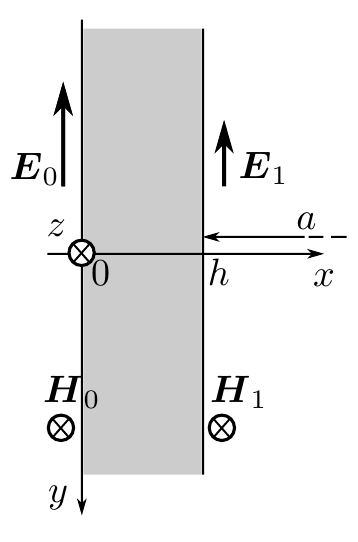
\includegraphics[width=0.28\textwidth]{stenka.png}
\end{center}
\caption{Поле в стенке циллиндра}
\label{img2}
\end{wrapfigure}

Поле внутри тонкой стенки цилиндра («экрана») описывается уравнением скин-эффекта (уравнением диффузии поля) в плоской геометрии (рис. \ref{img2}). Поместим начало отсчёта на внешнюю поверхность цилиндра и направим ось $x$ к оси системы, и запишем дифференциальное уравнение для комплексной амплитуды магнитного поля:

\[ \frac{d^2H}{dx^2} = i \omega \sigma \mu_0 H \]

для медного цилиндра можно положить $\mu \approx 1$).

Граничные условия зададим в виде

\[ H(0) = H_0 \text{, } H(h) = H_1. \]

Здесь $H_0$ — амплитуда колебаний магнитного поля на внешней границе цилиндра. Её значение определяется только током в обмотке соленоида, и совпадает с полем внутри соленоида в отсутствие цилиндра. Величина $H_1$ также поддаётся непосредственному измерению — это амплитуда колебаний однородного поля внутри цилиндра. Поля $H_0$
и $H_1$ не являются независимыми — они связаны через решение уравнений поля вне проводника, т. е. внутри «экрана».

Решение дифференциального уравнение ищем в виде

\[ H(x) = A e^{\alpha x} + B e^{-\alpha x}, \]

где $A$, $B$ -  определяемые из граничных условий константы,

\[ \alpha = \sqrt{i \omega \sigma \mu_0} = \frac{1 + i}{\delta} = \frac{\sqrt{2}}{\delta} e^{i \pi/4} \]

-- один из корней уравнения , $\delta$ — глубина скин-слоя

\[ \delta = \sqrt{\frac{2}{\omega \sigma \mu_0}}. \]

Здесь мы имеем дело уже не с полупространством, а с конечной областью в виде плоского слоя $h$, поэтому решение должно содержать оба корня.

Первое условие даёт $A + B = H_0$, что позволяет исключить $A$ из формулы:

\[ H(x) = H_0 e^{- \alpha x} + 2B \sinh{\alpha x}. \]

Выразим электрическое поле из закона Ампера. В одномерном случае

\[ E(x) = \frac{1}{\sigma} \frac{dH}{dx} = \frac{\alpha}{\sigma}(-H_0 e^{-\alpha x} + 2B \cosh{\alpha x}). \]

Далее положим $x = h$ и, исключив константу $B$, получим после преобразований связь между $H_0$ и $H_1$:

\[ H1 = \frac{H_0}{\cosh{\alpha h} + \frac{1}{2} \alpha a \sinh{ah}}. \]

Рассмотрим предельные случаи этой формулы.

\begin{enumerate}
    \item При \textit{малых частотах} толщина скин-слоя превосходит толщину цилиндра $h \ll \delta$. Тогда $|ah|\ll 1$, поэтому $\cosh{ah} \approx 1$, $\sinh{ah} \approx ah$ и

    \[ H_1 \approx \frac{H_0}{1 + i\frac{ah}{\delta^2}}. \]
    
    Заметим, что величина $\frac{ah}{\delta^2}$ в общем случае не мала, поскольку при $h \ll a$ возможна ситуация $h \ll \delta \ll a$. Отношение модулей амплитуд здесь будет равно
    
    \[ \frac{|H_1|}{|H_0|} = \frac{1}{\sqrt{1 + (\frac{ah}{\delta^2})^2}} = \frac{1}{\sqrt{1+\frac{1}{4}(a h \sigma \mu_0 \omega)^2}}. \]
    
    При этом колебания $H_1$ отстают по фазе от $H_0$ на угол $\psi$, определяемый равенством
    
    \[ tg(\psi) = \frac{ah}{\delta^2}. \]

    \item При достаточно больших частотах толщина скин-слоя станет меньше толщины стенки: $\delta \ll h$. Тогда $ah \gg 1$ и $\alpha a \gg 1$, $\sinh{ah} \approx \cosh{ah} \approx \frac{1}{2} e^{\alpha h}$. В итоге получим

    \[ \frac{H_1}{H_0} = \frac{4}{\alpha a} e^{-\alpha h} = \frac{2\sqrt{2} \delta}{a} e^{-\frac{h}{\delta}}e^{-i(\frac{\pi}{4} + \frac{h}{\delta})}. \]

    Как видно из формулы, в этом пределе поле внутри цилиндра по модулю в $\frac{2\sqrt{2} \delta}{a} e^{-\frac{h}{\delta}}$ раз меньше, чем снаружи, и, кроме того, запаздывает по фазе на

    \[ \psi = \frac{\pi}{4} + \frac{h}{\delta} = \frac{\pi}{4} + h \sqrt{\frac{\omega \sigma \mu_0}{2}}. \]

    На рис. \ref{img3} схематично изображено распределение магнитного поля от координаты в двух рассмотренных предельных случаях.

    \begin{figure}[h]
        \begin{center}
    		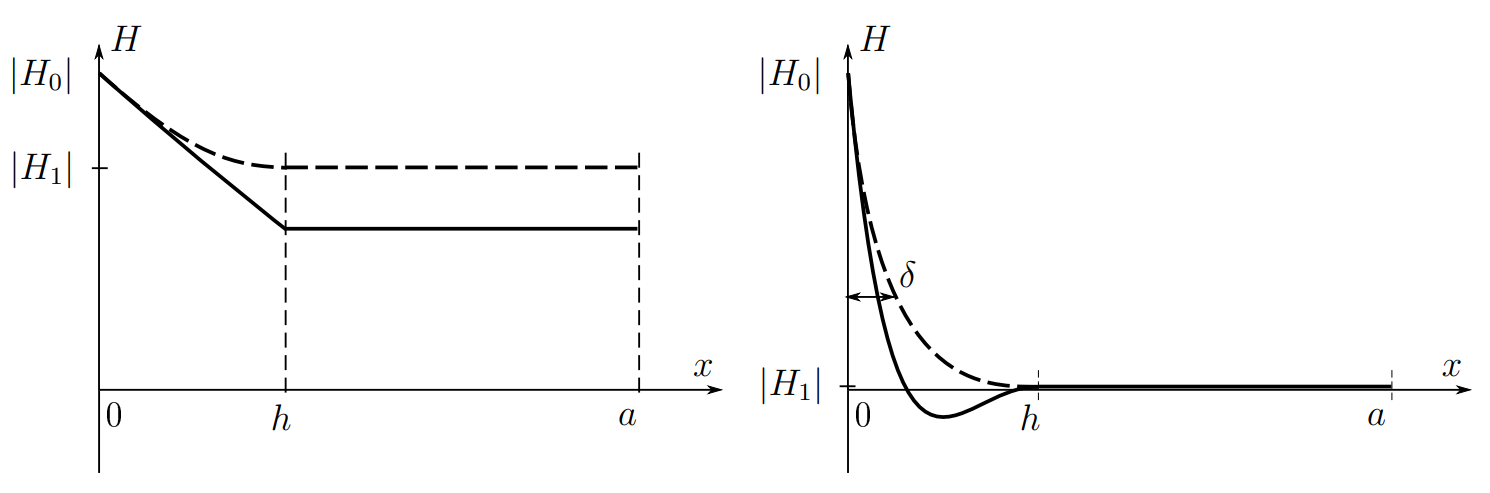
\includegraphics[width=16cm]{graf_teor.png}
        \end{center}
    	\caption{Распределение амплитуды колебаний магнитного поля (пунктир) и его мгновенного значения при некотором $t$ (сплошная) в зависимости от расстояния до внешней стенки цилиндра.
Слева случай низких частот ($\delta \gg h$), справа — скин-эффект при высоких частотах ($\delta \ll h$)}
    \label{img3}
    \end{figure}

\end{enumerate}

\subsection{Экспериментальная установка}

Схема экспериментальной установки для исследования скин–эффекта в полом цилиндре изображена на рис. \ref{img4}.


\begin{figure}[h]
        \begin{minipage}[h]{1\linewidth}
    	\center{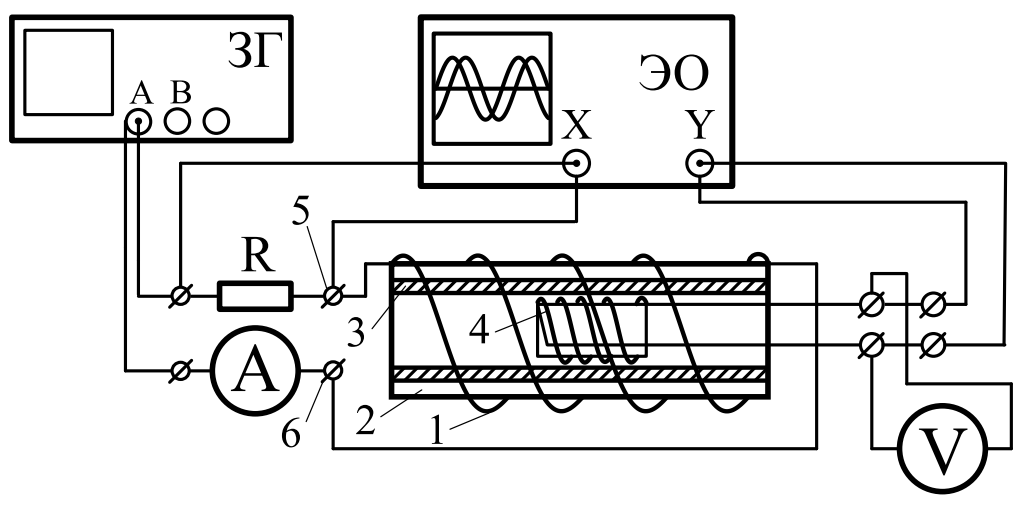
\includegraphics[width=0.8\linewidth]{ustanovka.png}}
    	\caption{Экспериментальная установка для изучения скин-эффекта}
            \label{img4}
        \end{minipage}
        \begin{minipage}[h]{1\linewidth}
    	\center{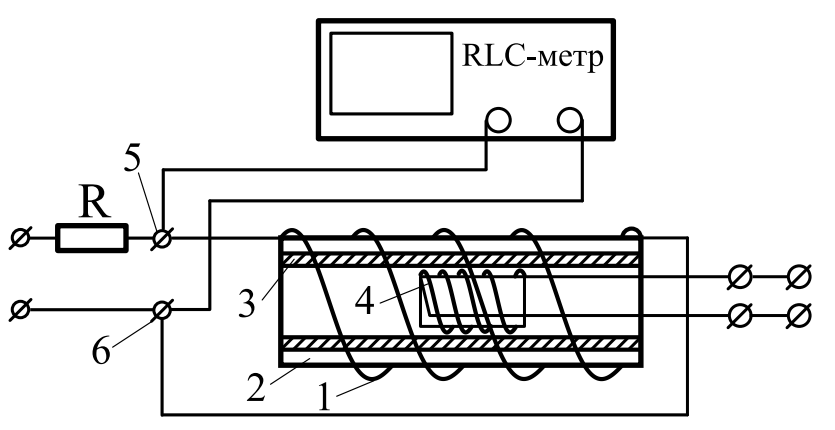
\includegraphics[width=0.8\linewidth]{ustanovka_2.png}}
    	\caption{Экспериментальная установка для изучения скин-эффекта}
            \label{img5}
        \end{minipage}
    \end{figure}
	

Переменное магнитное поле создается с помощью соленоида 1, намотанного на цилиндрический каркас 2 из поливинилхлорида, который подключается к генератору сигналов (канал А). Внутри каркаса расположен медный экран 3 в виде полого цилиндра (актуальные параметры экрана указаны на установке). Действующее значение переменного тока в цепи соленоида измеряется цифровым амперметром «А». Действующее значение переменного напряжения на измерительной катушке 4 измеряется цифровым вольтметром «V». В качестве амперметра и вольтметра используются два мультиметра.
Для измерения сдвига фаз между током в цепи соленоида и напряжением на измерительной катушке используется двухканальный осциллограф. На канал $'Y'$ осциллографа подается напряжение с измерительной катушки, а на канал $'X'$ — напряжение с резистора $R$, которое пропорционально току в цепи соленоида.

Схема экспериментальной установки для нахождения проводимости $\sigma$ по изменению индуктивности катушки $L$ изображена на рис. \ref{img5}. $RLC-метр$, измеряющий индуктивность, подключается к катушке 1 через клеммы 5 и 6 на панеле установки. Другие приборы при этом должны быть отсоединены от цепи, т.к. $RLC-метр$ измеряет индуктивность активным образом.

\subsection{Ход работы}

\begin{enumerate}
    \item По известным параметрам установки, приняв проводимость меди для оценки равной $\sigma \approx 5 \cdot 10^7 \frac{\text{Сименс}}{\text{м}}$, а $\mu_0 \approx 1.256 \cdot 10^{-6} \frac{\text{Гн}}{\text{м}}$, рассчитаем частоту $\nu_{h}$, при которой толщина стенок экрана равна скиновской длине $h = \delta$.

    \textbf{Параметры нашей установки:} $a = 22.5 \text{мм}$,  $h = 1.5 \text{мм}$.

    \begin{figure}[!h]
        \centering
        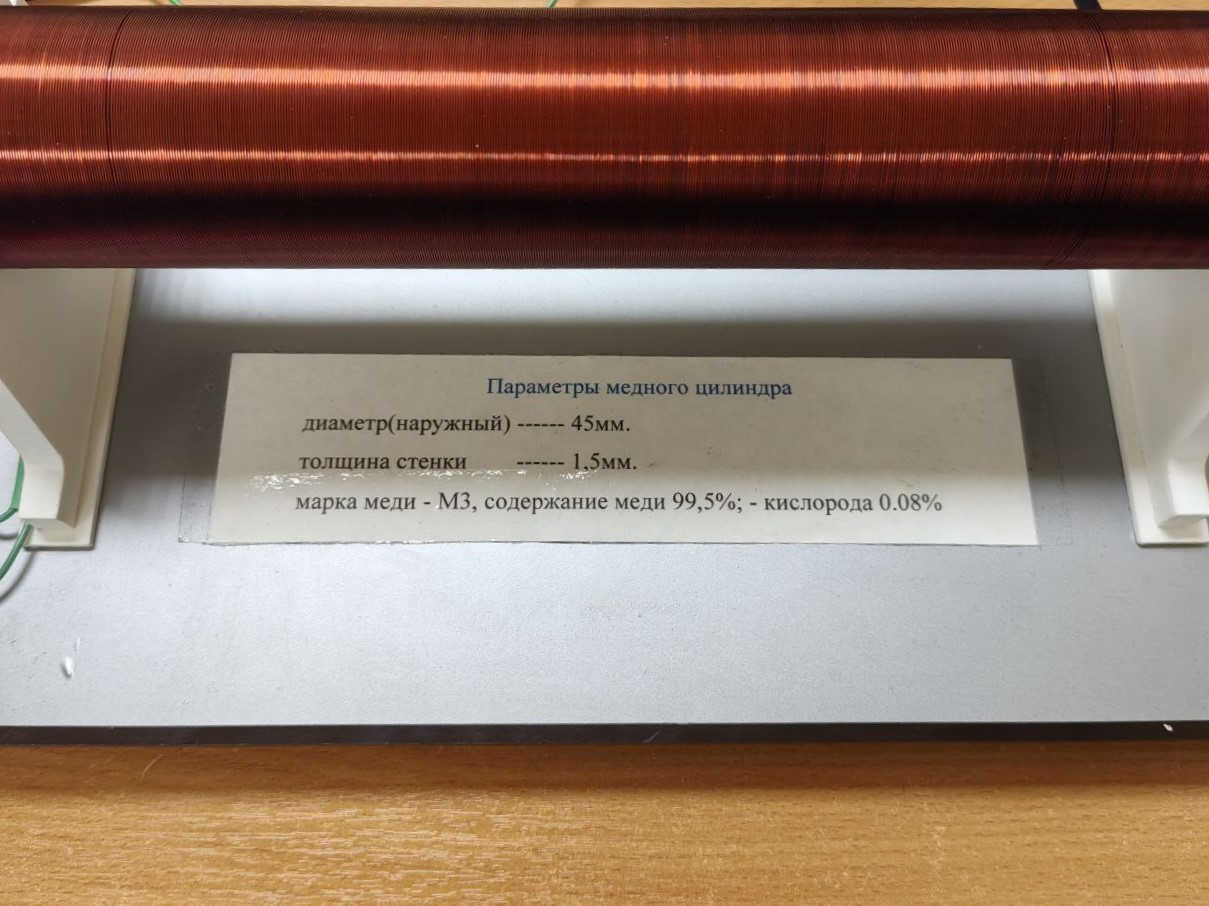
\includegraphics[width=10cm]{7.jpg}
        \label{graf1}
    \end{figure}

    \[ \delta = \sqrt{\frac{2}{\omega \sigma \mu_0}} \Leftrightarrow \omega = \frac{2}{\delta^2 \sigma \mu_0} \Leftrightarrow 2 \pi \nu = \frac{2}{\delta^2 \sigma \mu_0} \Leftrightarrow \nu = \frac{1}{\pi \delta^2 \sigma \mu_0} \] \[ \Rightarrow \nu = \frac{1}{3.14 \cdot (1.5 \cdot 10^{-3})^2 \cdot 5 \cdot 10^7 \cdot 1.256 \cdot 10^{-6}} = 2252.724 \text{ Гц}. \]

    \item Соберём установку согласно схеме на рис. \ref{img4} и настроим приборы, следуя указаниям пособия. Установим начальную частоту сигнала генератора $\nu_0 \approx 0.01 \nu_{h} \approx 22.53 \text{ Гц}$, а амплитуду выходного сигнала на генераторе — согласно приложению
    
    \item В области низких частот ($\nu_0 \approx 0.01 \nu_{h}$ до $\nu_0 \approx 0.05 \nu_{h}$) получиим зависимость отношения
    $\xi = \frac{U}{\nu I}$ от частоты $\nu$.
    
    Для этого измерим силу тока в цепи соленоида и напряжение на измерительной катушке для не менее 10 значений частоты $\nu$ в выбранном диапазоне. Согласно формулам величина $\xi$ прямо пропорциональна коэффициенту ослабления магнитного поля внутри экрана относительно поля снаружи: $\xi\xi_0 = \frac{H_1}{H_0}.$

    Результаты занесём в таблицу \ref{tab1}.

    \begin{table}[h]
	\centering
		\begin{tabular}{|c|c|c|c|}
			\hline
                $N$ & $\nu, \text{Гц}$ &  $I, \text{мА}$ & $U, \text{В}$ \\ \hline
                1 & 22.53 & 231.3 & 0.0723 \\ \hline
                2 & 33.79 & 229.25 & 0.106 \\ \hline
                3 & 45.05 & 226.2 & 0.1373 \\ \hline
                4 & 56.32 & 222.65 & 0.166 \\ \hline
                5 & 63.08 & 220.15 & 0.1812 \\ \hline
		\end{tabular}
            \hspace{.02\textwidth}
            \begin{tabular}{|c|c|c|c|}
			\hline
                $N$ & $\nu, \text{Гц}$ &  $I, \text{мА}$ & $U, \text{В}$ \\ \hline
                6 & 67.58 & 218.72 & 0.191 \\ \hline
                7 & 79.85 & 214.76 & 0.214 \\ \hline
                8 & 90.11 & 210.82 & 0.233 \\ \hline
                9 & 100.37 & 207.02 & 0.2503 \\ \hline
                10 & 112.64 & 203.38 & 0.265 \\ \hline
		\end{tabular}
	\caption{Результаты измерений}
        \label{tab1}
    \end{table}

    \item  Исследуем зависимость величины $\varepsilon$ и фазового сдвига $\psi$ от частоты $\nu$ при низких частотах в диапазоне от $0.05\nu_h$ до $0.5\nu_h$. Для этого получим статичную и удобную для измерения картинку на экране осциллографа и измерим разность фаз между напряжениями на резисторе и на катушке для не менее 15 значений частоты $\nu$ в выбранном диапазоне, а также силу тока в цепи соленоида и напряжение на измерительной катушке.

    Результаты занесём в таблицу \ref{tab2}.

    \begin{table}[h]
        \centering
        \begin{tabular}{|c|c|c|c|c|}
			\hline
                $N$ & $\nu, \text{Гц}$ &  $I, \text{мА}$ & $U, \text{В}$ & $\Delta \varphi \cdot \pi$ \\ \hline
                1 & 112.64 & 202.63 & 0.265 & 1.38 \\ \hline
                2 & 135.16 & 196.23 & 0.288 & 1.29 \\ \hline
                3 & 157.69 & 190.69 & 0.306 & 1.33 \\ \hline
                4 & 180.22 & 186.05 & 0.319 & 1.4  \\ \hline
                5 & 202.74 & 182.18 & 0.329 & 1.12 \\ \hline
                6 & 225.27 & 178.91 & 0.336 & 1.11 \\ \hline
                7 & 281.59 & 172.74 & 0.348 & 1.2  \\\hline
                8 & 337.91 & 168.34 & 0.353 & 1.15 \\ \hline
		\end{tabular}
            \hspace{.02\textwidth}
            \begin{tabular}{|c|c|c|c|c|}
			\hline
                $N$ & $\nu, \text{Гц}$ &  $I, \text{мА}$ & $U, \text{В}$ & $\Delta \varphi \cdot \pi$ \\ \hline
                9 & 394.22 & 164.94 & 0.356 & 1.13 \\ \hline
                10 & 450.54 & 162.10 & 0.356 & 1.15 \\ \hline
                11 & 563.17 & 157.23 & 0.353 & 1.1 \\ \hline
                12 & 675.81 & 152.77 & 0.347 & 1.06 \\ \hline
                13 & 788.44 & 148.40 & 0.340 & 1.06 \\ \hline
                14 & 901.08 & 144.08 & 0.331 & 1.01 \\ \hline
                15 & 1126.35 & 135.28 & 0.313 & 1.0 \\ \hline
		\end{tabular}
        \caption{Результаты измерений в диапазоне низких частот}
        \label{tab2}
    \end{table}

    \item Повторим измерения пункта $4$ при высоких частотах в диапазоне от $0.5\nu_h$ до $15\nu_h$.

    Результаты занесём в таблицу \ref{tab3}.

    \begin{table}[h]
        \centering
        \begin{tabular}{|c|c|c|c|c|}
			\hline
                $N$ & $\nu, \text{Гц}$ &  $I, \text{мА}$ & $U, \text{В}$ & $\Delta \varphi \cdot \pi$ \\ \hline
                1 & 1352.82 & 126.48 & 0.293 & 0.97 \\ \hline
                2 & 1916.49 & 106.70 & 0.247 & 0.93 \\ \hline
                3 & 2592.91 & 87.80 & 0.202 & 0.93 \\ \hline
                4 & 3156.58 & 75.73 & 0.173 & 0.85 \\ \hline
                5 & 3720.25 & 66.27 & 0.150 & 0.87 \\ \hline
                6 & 4283.93 & 52.59 & 0.116 & 0.86 \\ \hline
                7 & 4847.61 & 47.45 & 0.104 & 0.8 \\ \hline
                8 & 5411.28 & 41.92 & 0.09 & 0.82 \\ \hline
                9 & 5974.95 & 38.57 & 0.082 & 0.81 \\ \hline
		\end{tabular}
            \hspace{.02\textwidth}
            \begin{tabular}{|c|c|c|c|c|}
			\hline
                $N$ & $\nu, \text{Гц}$ &  $I, \text{мА}$ & $U, \text{В}$ & $\Delta \varphi \cdot \pi$ \\ \hline
                10 & 6538.63 & 35.66 & 0.075 & 0.81 \\ \hline
                11 & 7102.31 & 33.11 & 0.068 & 0.77 \\ \hline
                12 & 7665.98 & 30.85 & 0.063 & 0.76 \\ \hline
                13 & 8229.65 & 28.84 & 0.058 & 0.75 \\ \hline
                14 & 8793.33 & 27.03 & 0.053 & 0.74 \\ \hline
                15 & 9357.11 & 25.40 & 0.049 & 0.72 \\ \hline
                16 & 9920.68 & 23.92 & 0.046 & 0.71 \\ \hline
                17 & 10484.35 & 22.56 & 0.043 & 0.69 \\ \hline
                18 & 11048.03 & 21.51 & 0.039 & 0.7 \\ \hline
		\end{tabular}
        \caption{Результаты измерений в диапазоне высоких частот}
        \label{tab3}
    \end{table}

    \item Исследуем зависимость индуктивности катушки $L$ от частоты $\nu$. Для этого соберём схему, изображенную на рисунке \ref{img5}, и измерим с помощью RLC-метра индуктивность катушки при различных частотах (от минимально возможной для данной модели RLC-метра $\nu_{min}$ до $1.5 \nu_h$).

     Результаты занесём в таблицу \ref{tab4}.

    \begin{table}[h]
        \centering
        \begin{tabular}{|c|c|c|}
			\hline
                $N$ & $\nu, \text{Гц}$ &  $L, \text{мГн}$ \\ \hline
                1 & 50 & 9.99 \\ \hline
                2 & 250 & 5.38 \\ \hline
                3 & 500 & 3.69 \\ \hline
                4 & 750 & 3.25 \\ \hline
                5 & 1000 & 3.09 \\ \hline
                6 & 1500 & 2.96 \\ \hline
                7 & 2000 & 2.91 \\ \hline
                8 & 2500 & 2.90 \\ \hline
		\end{tabular}
            \hspace{.02\textwidth}
            \begin{tabular}{|c|c|c|}
			\hline
                $N$ & $\nu, \text{Гц}$ &  $L, \text{мГн}$ \\ \hline
                9 & 3000 & 2.89 \\ \hline
                10 & 5000 & 2.88 \\ \hline
                11 & 6000 & 2.89 \\ \hline
                12 & 7500 & 2.9 \\ \hline
                13 & 10000 & 2.95 \\ \hline
                14 & 12000 & 3.02 \\ \hline
                15 & 15000 & 3.18 \\ \hline
                16 & 20000 & 3.62 \\ \hline
		\end{tabular}
        \caption{Результаты измерений индуктивности катушки от частоты}
        \label{tab4}
    \end{table}
\end{enumerate}

\newpage

\subsection{Обработка результатов}

\begin{enumerate}
        \item В области низких частот толщина скин-слоя превосходит толщину образца $ \delta \gg h$, получаем
	
        \[ \left(\frac{|H_1|}{|H_0|}\right)^2 = \left(\frac{\xi}{\xi_0}\right)^2 \approx \frac{1}{1+\left(\frac{ah}{\delta^2}\right)^2} = \frac{1}{1 + \left(\pi ah\nu\mu_0\sigma\right)^2} \]
	Тогда: 
	\begin{equation*}
		\frac{1}{\xi^2}=k\nu^2 + b \text{, где } k=\left(\frac{\pi a h \sigma \mu_0}{\xi_0}\right)^2\text{, } b = \frac{1}{\xi_0^2}.
	\end{equation*}
 
    По результатам измерений в области низких частот  постройте график $\frac{1}{\xi^2}=f(\nu^2)$. График представлен на рисунке \ref{graf1}.

    \begin{figure}[h]
        \centering
        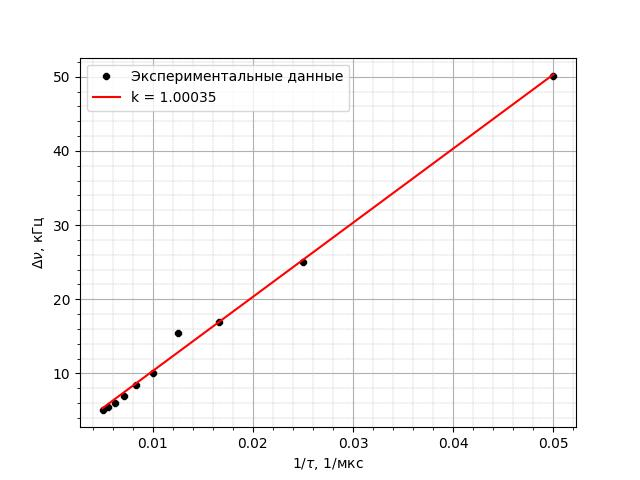
\includegraphics[width=18cm]{image1.jpg}
        \caption{Графическая зависимость $\frac{1}{\xi^2}=f(\nu^2)$}
        \label{graf1}
    \end{figure}

    Аппроксимируем с помощью метода наименьшего квадрата, погрешности получаем благодаря функции $curvefit$. Экстраполируем к точке $\nu = 0$, соответствующей $\frac{|H_1|}{|H_0|} = 1$:

    \[ b = (5102.45 \pm 26.49) \frac{\text{Гц}^2}{\text{Ом}^2} \text{ }(\varepsilon = 0.51 \%)\Longrightarrow \xi_0 = \frac{1}{\sqrt{b}} = (13.99 \pm 0.07) \cdot 10^{-3} \text{ } \frac{\text{Ом}}{\text{Гц}}.
    \]

    По угловому коэффициенту зависимости рассчитаем проводимость меди:

    \[ k = (182.77 \pm 0.08) \cdot 10^{-3} \frac{\text{Гц}^2}{\text{Ом}^2} \text{ }(\varepsilon = 0.04 \%)\Longrightarrow \] \[ k=\left(\frac{\pi a h \sigma \mu_0}{\xi_0}\right)^2 \Leftrightarrow \sigma = \frac{\sqrt{k}\xi_0}{ah\mu_0\pi} = \frac{\sqrt{0.18277} \cdot 0.01399}{\pi\cdot1.5\cdot22.5\cdot1.256 \cdot10^{-12}} \approx (4.491 \pm 0.002 )\cdot 10^7 \text{ }\frac{\text{Сименс}}{\text{м}}. \]

\newpage

    \item Построим график зависимости фазового сдвига, измеренного в пункте 4, $\tg \psi = f(\nu)$ от частоты. 

    \begin{figure}[!h]
        \centering
        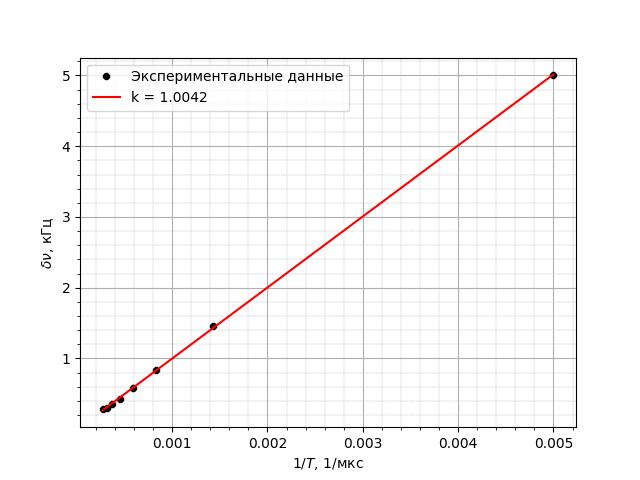
\includegraphics[width=18cm]{image2.jpg}
        \caption{Графическая зависимость $tg \psi=f(\nu)$}
        \label{graf1}
    \end{figure}

    Учтём, что на входной канал $Y$ осциллографа подаётся сигнал с измерительной катушки, который пропорционален не полю внутри экрана,
    а его производной по времени, а это означает, что появляется дополнительный сдвиг по фазе на $\frac{\pi}{2}$. Поэтому измеренный по экрану осциллографа сдвиг по фазе между двумя синусоидами будет на $\frac{\pi}{2}$ больше фазового сдвига между магнитными полями вне и внутри экрана: $\varphi = \frac{\pi}{2} + \psi$.

    Аппроксимируем прямой линейный участок графика, и по её наклону определим коэффициент проводимости $\sigma$.

    \[ tg \psi = \frac{ah}{\delta^2} \Leftrightarrow tg \psi = k\nu \text{, где } k = ah\sigma\mu_0\pi. \]
    \[ k = (6.548 \pm 1.065) \cdot 10^{-3} \text{ Гц}^{-1} \text{ }(\varepsilon = 16 \%) \Longrightarrow \] \[ \sigma = \frac{k}{ah\mu_0\pi} = \frac{6.548\cdot 10^{-3}}{1.5\cdot22.5\cdot1.256\cdot\pi\cdot10^{-12}} = (4.9 \pm 0.8) \cdot 10^{7}\text{ }\frac{\text{Сименс}}{\text{м}}.  \]

    \item Построим график частотной зависимости фазового сдвига, измеренной в пунктах 4 и 5, $\psi - \frac{\pi}{4} = f(\sqrt{\nu})$).
    Проведём прямую, проходящую через начало координат, которая будет касаться экспериментальной кривой при больших частотах(линейный участок графика при $\nu \gg \nu_{h}$).
    По наклону этой прямой вычислите значение проводимости $\sigma$ материала экрана.

    \[ \psi - \frac{\pi}{4} = k\cdot\sqrt{\nu} \text{, где } k = \sqrt{\pi\sigma\mu_0}. \]
    \[ k = (21.23 \pm 0.72) \cdot 10^{-3} \frac{1}{\sqrt{\text{Гц}}} (\varepsilon = 3.39 \%) \Longrightarrow \] \[ \sigma = \frac{k^2}{\pi h^2\mu_0} = \frac{(21.23 \cdot 10^{-3})^2}{\pi \cdot 1.5^{2} \cdot 1.256 \cdot 10^{-12}} = (5.077 \pm 0.172) \cdot 10^{7}\text{ }\frac{\text{Сименс}}{\text{м}}. \]

    \begin{figure}[!h]
        \centering
        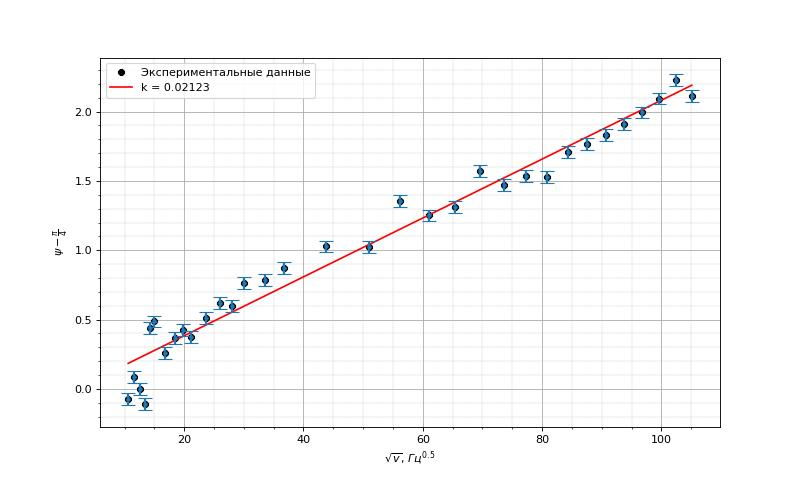
\includegraphics[width=18cm]{image3.jpg}
        \caption{Графическая зависимость $\psi - \frac{\pi}{4} = f(\sqrt{\nu})$}
        \label{graf1}
    \end{figure}

    \item Построим график зависимости индуктивности катушки от частоты $L(\nu)$. Определм максимальное и минимальное значения индуктивности.

    \begin{figure}[!h]
        \centering
        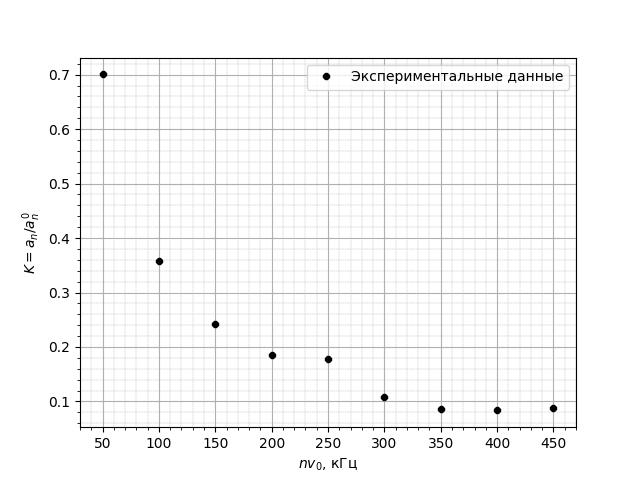
\includegraphics[width=16cm]{image4.jpg}
        \caption{Графическая зависимость $L(\nu)$}
        \label{graf1}
    \end{figure}

    \[ L_{max} = 9.99 \text{ мГн},  L_{min} = 2.88 \text{ мГн.}\]

    Построим график зависимости $(L_{max} - L)/(L - L_{min})$ от $\nu^2$ и аппроксимируем его прямой, проходящей через начало координат. По углу наклона прямой определим проводимость материала.

    \begin{figure}[!h]
        \centering
        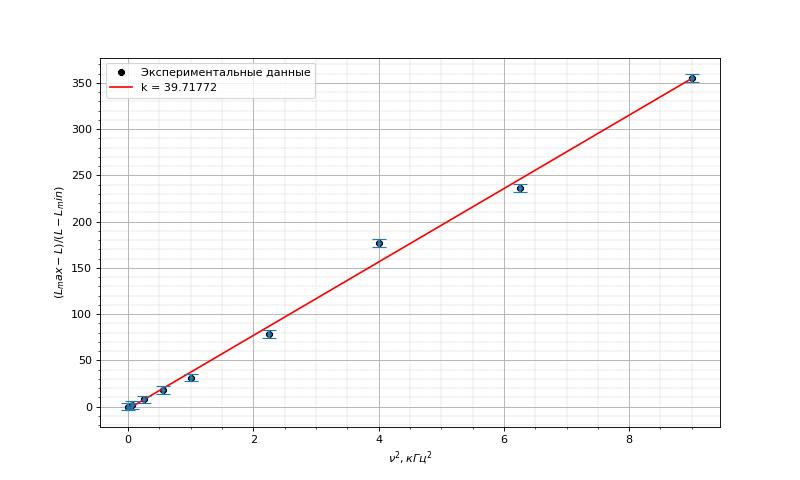
\includegraphics[width=18cm]{image5.jpg}
        \caption{Графическая зависимость $\frac{L_{max} - L}{L - L_{min}}(\nu^2)$}
        \label{graf1}
    \end{figure}

    \[ \frac{L_{max} - L}{L - L_{min}} = k\cdot\nu^2 \text{, где } k = (\pi ah\mu_0\sigma)^2. \]
    \[ k = (39.72 \pm 1.06) \frac{1}{\text{кГц}^2} (\varepsilon = 2.67 \%) \Longrightarrow \] \[ \sigma = \frac{\sqrt{k}}{\pi ah\mu_0} = \frac{\sqrt{39.72 \cdot 10^{-6}}}{\pi \cdot 22.5 \cdot 1.5 \cdot 1.256 \cdot 10^{-12}} = (4.73 \pm 0.13) \cdot 10^{7}\text{ }\frac{\text{Сименс}}{\text{м}}. \]

    \item Составим таблицу, внеся в нее все полученные значения проводимости материала экрана (4-мя способами) и сравним с табличным значением.

    \begin{table}[h]
        \centering
        \begin{tabular}{|c|c|c|c|}
			\hline
                $N$ & $\sigma \cdot 10^7, \frac{\text{Сименс}}{\text{м}}$ &  $\varepsilon, \%$ & $\varepsilon_{\text{отк}}, \%$ \\ \hline
                табл & 5.66 & - & - \\ \hline
                1 & 4.49 & 0.04 & 20 \\ \hline
                2 & 4.9 & 16 & 13 \\ \hline
                3 & 5.077 & 3.39 & 10 \\ \hline
                4 & 4.73 & 2.67 & 16 \\ \hline
		\end{tabular}
        \caption{Результаты измерений удельной проводимости меди}
        \label{tab5}
    \end{table}

    \item Используя полученное значение коэффициента $\xi_0$, рассчитаем экспериментальные значения коэффициентов ослабления поля $|H_1|/|H_0|$ для всех измерений - экспериментальный коэффициент.
    
    Используя максимальный и минимальный коэффициенты проводимости $\sigma$, полученные
    ранее, рассчитаем теоретическую зависимость по общей формуле - теоретический коэффициент.

    Изобразим на графике теоретические и экспериментальные результаты для зависимости $\frac{|H_1|}{|H_0|}$ от $nu$ в логарифмическом масштабе по оси абсцисс.

    \begin{figure}[!h]
        \centering
        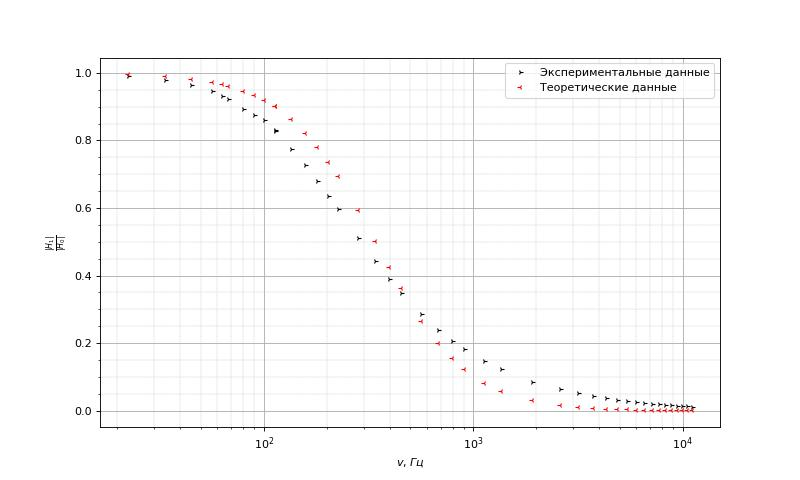
\includegraphics[width=18cm]{image6.jpg}
        \caption{Графическая зависимость $\frac{|H_1|}{|H_0|}(\nu)$}
        \label{graf1}
    \end{figure}
\end{enumerate}

\subsection{Обсуждение результатов и выводы}

В ходе этой работы мы измерили удельную проводимость медного цилиндра разными способами. Результаты измерений представлены в таблице $\ref{tab5}$. Полученные значения совпадают по порядку с теоретическим значением, однако немного меньше. Это может быть связано из-за приблиения о бесконечности цилиндра. Также на неточность измерений могла повлиять наводка поля в соединительных проводах.

Что касается коэффициентов ослабления поля, то из графика видно, что при малых частотах полученный коэффициент экспериментальным путём, меньше теоретического. При больших частотах картина противоположная, полученный коэффициент больше теоретического.

\newpage

\subsection{Приложения}

\begin{figure}[h]
    \begin{minipage}[h]{0.5\linewidth}
        \center{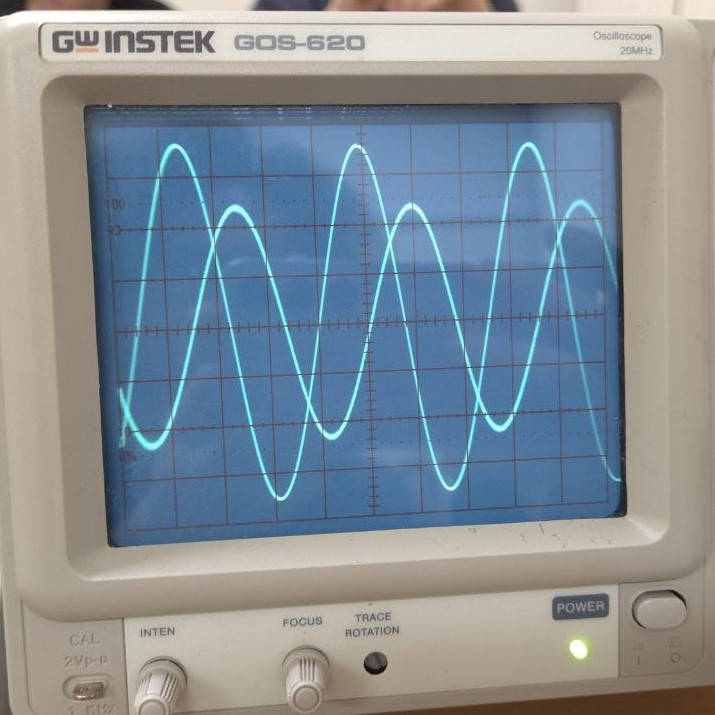
\includegraphics[width=0.7\linewidth]{1.jpg}}
    \end{minipage}
    \begin{minipage}[h]{0.5\linewidth}
        \center{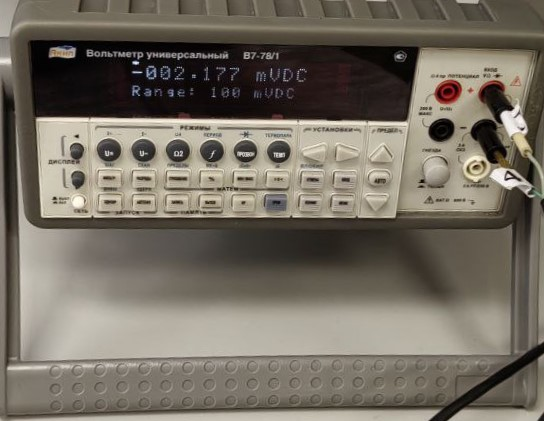
\includegraphics[width=0.7\linewidth]{2.jpg}}
    \end{minipage}
    \begin{minipage}[h]{0.5\linewidth}
        \center{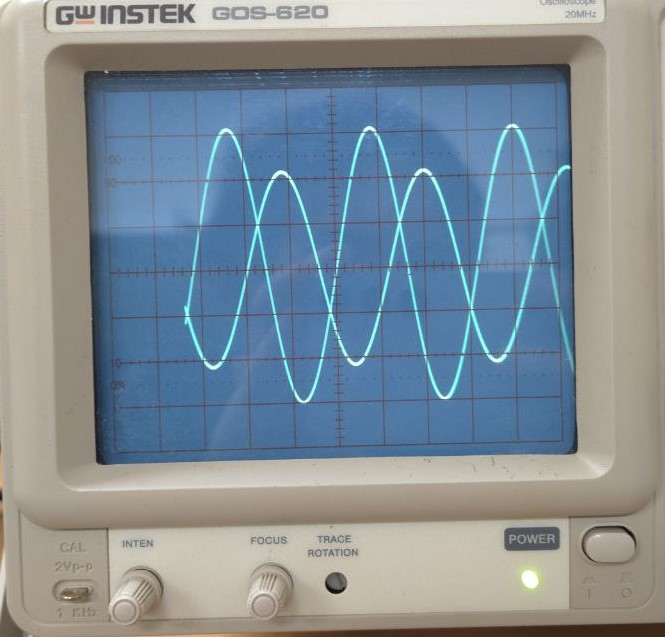
\includegraphics[width=0.7\linewidth]{3.jpg}}
    \end{minipage}
    \begin{minipage}[h]{0.5\linewidth}
        \center{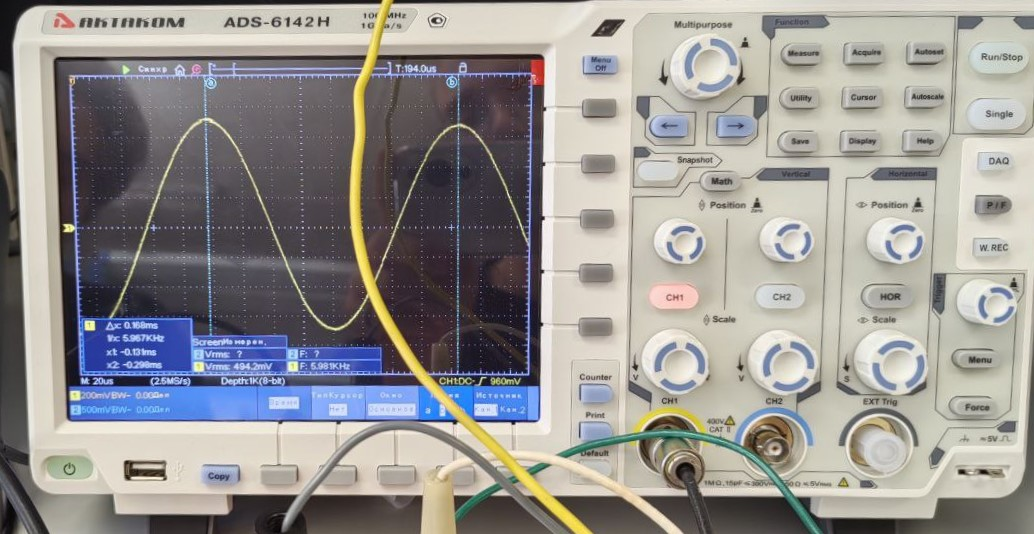
\includegraphics[width=0.7\linewidth]{4.jpg}}
    \end{minipage}
    \caption{Измерение сдвига фаз}
\end{figure}

\begin{figure}[h]
    \begin{minipage}[h]{0.5\linewidth}
        \center{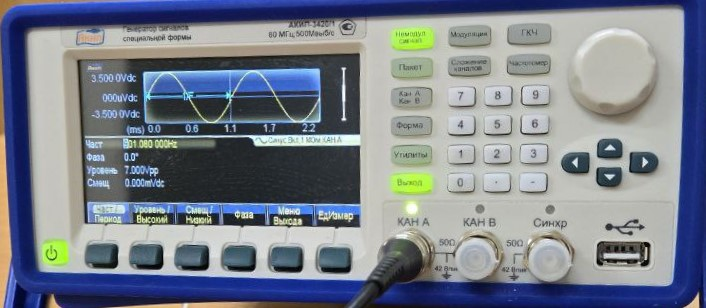
\includegraphics[width=0.7\linewidth]{11.jpg}}
    \end{minipage}
    \begin{minipage}[h]{0.5\linewidth}
        \center{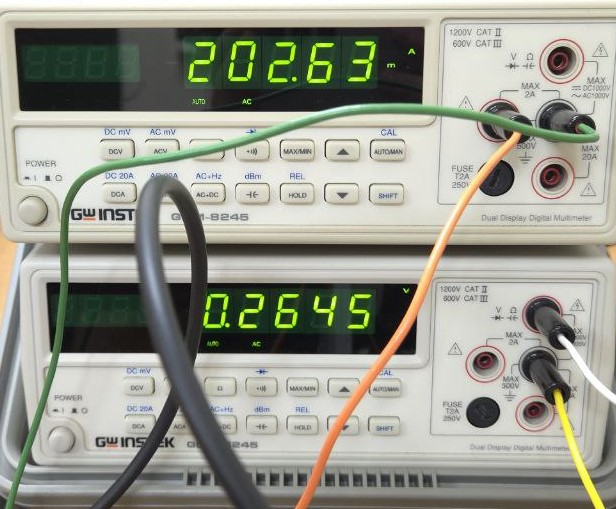
\includegraphics[width=0.7\linewidth]{8.jpg}}
    \end{minipage}
    \begin{minipage}[h]{0.5\linewidth}
        \center{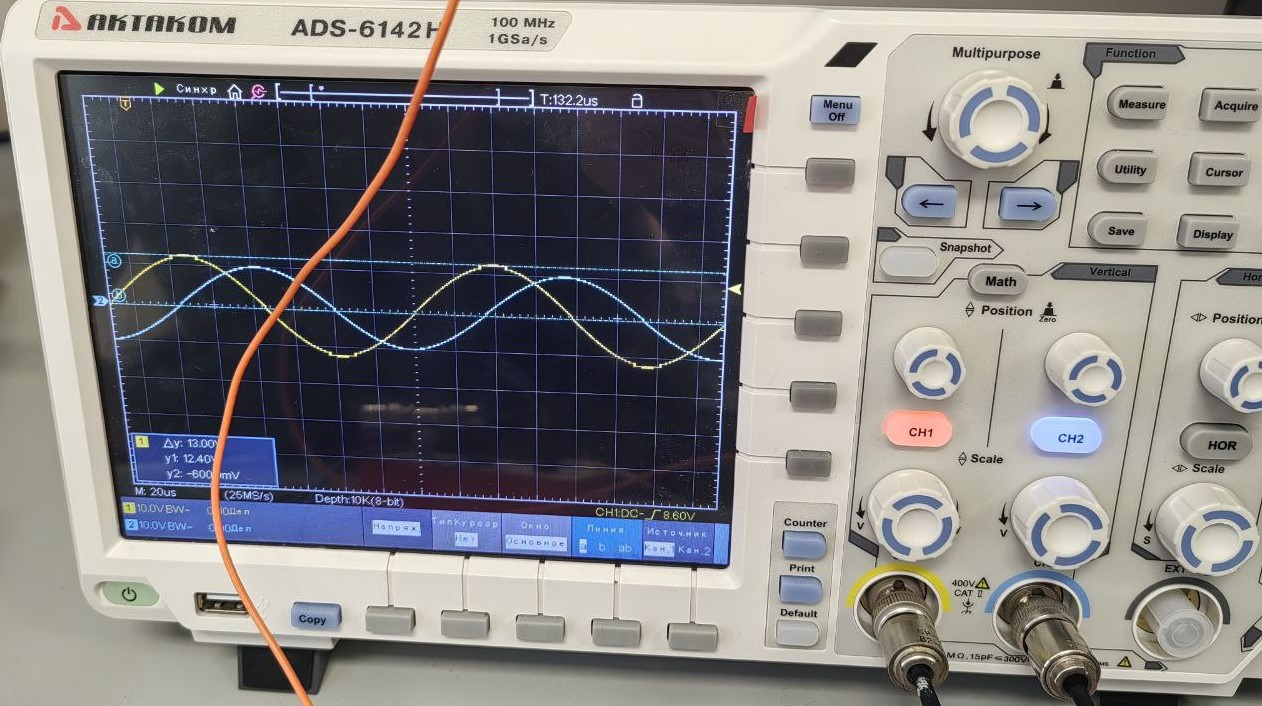
\includegraphics[width=0.7\linewidth]{9.jpg}}
    \end{minipage}
    \begin{minipage}[h]{0.5\linewidth}
        \center{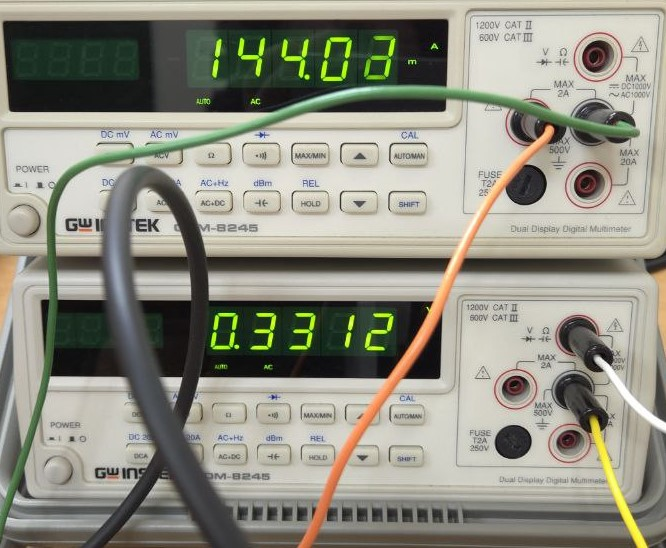
\includegraphics[width=0.7\linewidth]{10.jpg}}
    \end{minipage}
    \caption{Измерение тока и напряжение при разных частотах}
\end{figure}

\begin{figure}[h]
    \begin{minipage}[h]{0.5\linewidth}
        \center{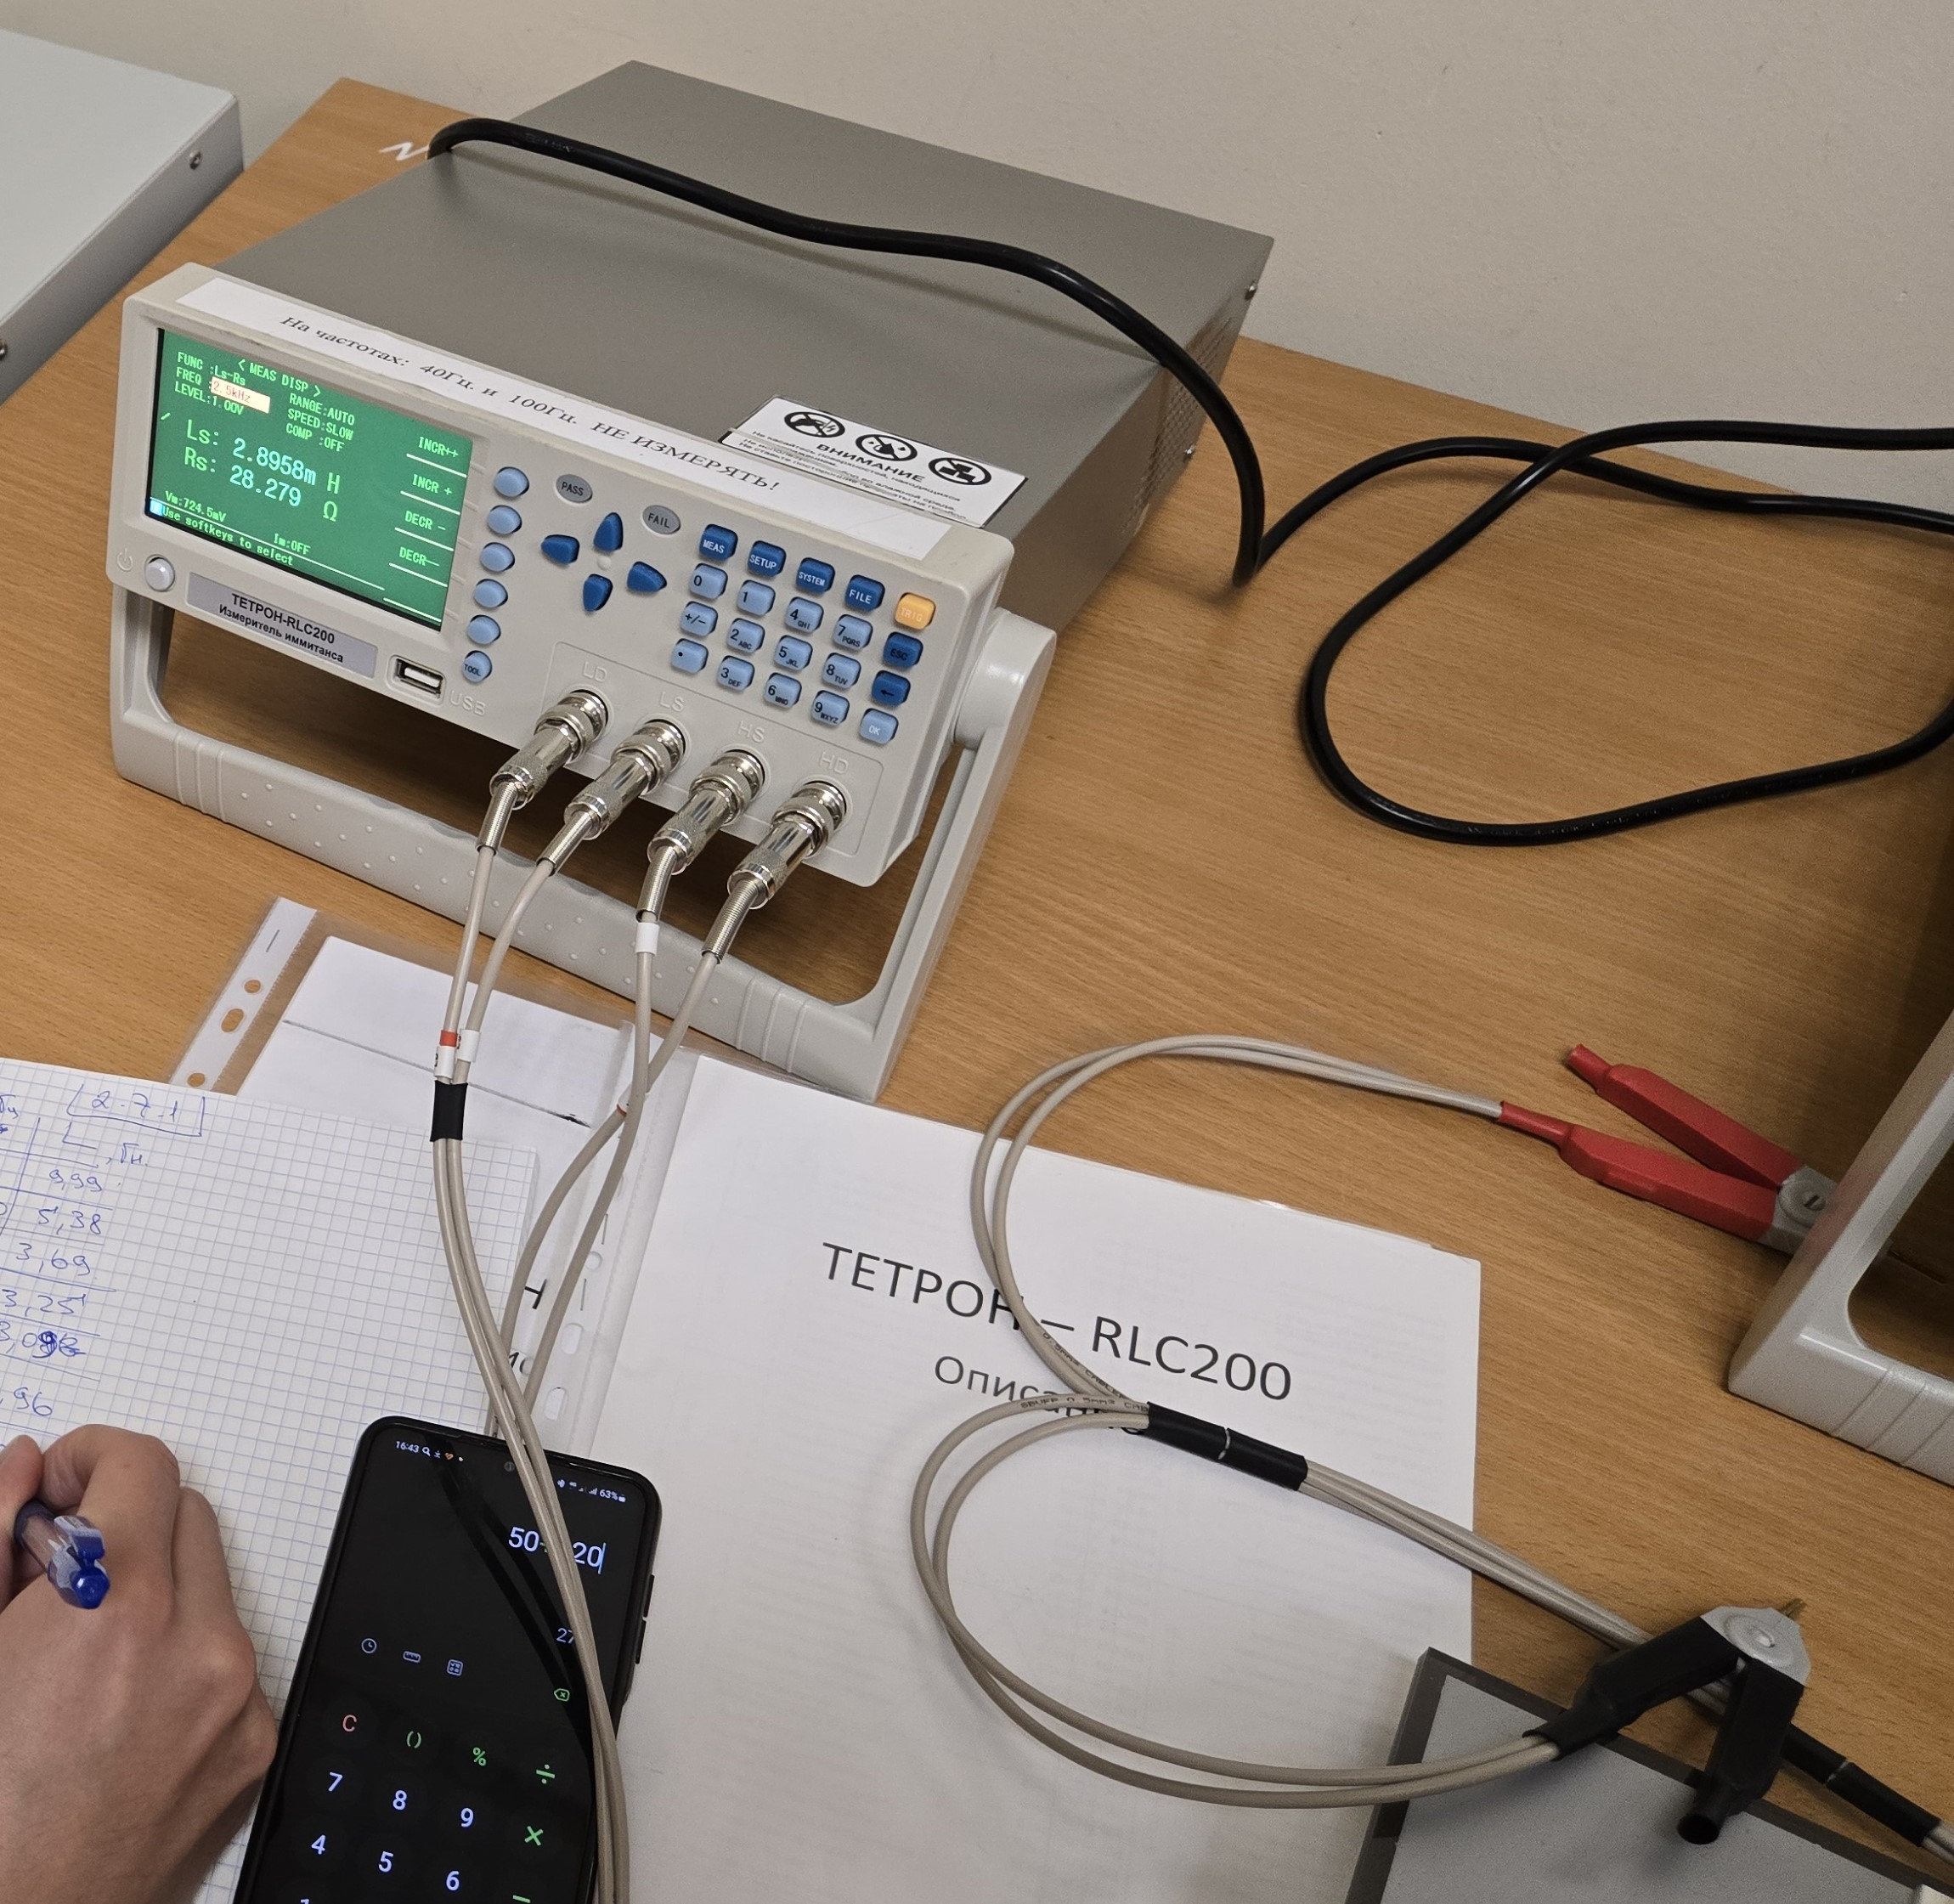
\includegraphics[width=0.9\linewidth]{5.jpg}}
    \end{minipage}
    \begin{minipage}[h]{0.5\linewidth}
        \center{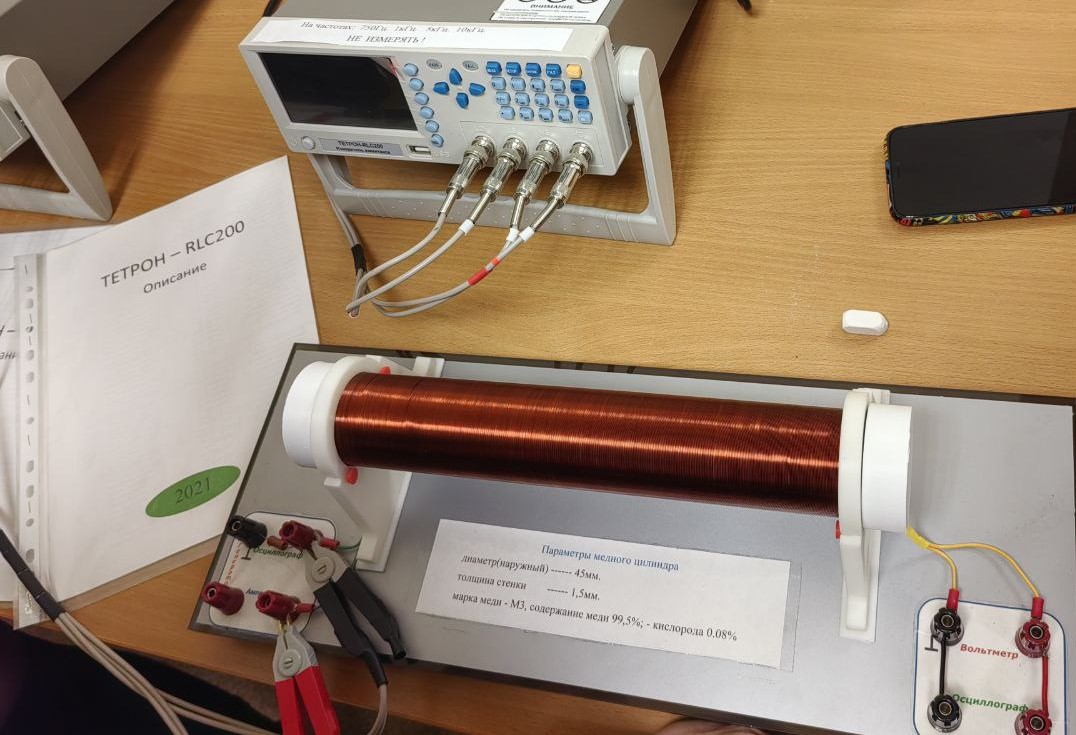
\includegraphics[width=0.9\linewidth]{6.jpg}}
    \end{minipage}
    \caption{Измерение зависимости индуктивности от частоты}
\end{figure}




\end{document}